%% FullCourse_10Lecs -- Lecture 6, Topic 6.3: Krusell--Smith + DeepHAM
%% Source: ./archive_pre_split/Lec06_HA_Models.tex (sections 6-7)
%% Pass B: layer in M2_T4_KS_DEQN refinements

%% Shared preamble for the FullCourse_10Lecs topic decks.
%%
%% Each topic .tex \input's this file, then defines its own \title, \date
%% override (if any), \graphicspath, and \begin{document}.
%%
%% Reconstructed verbatim from the inlined copy preserved in
%% Lec10_Case_Studies/Lec10_T8_Case6_DeepRamsey.tex (lines 23-190), which is
%% explicitly annotated there as "from ../shared_preamble.tex, copied verbatim".
%% Base preamble matches MiniCourse_8hr/Slides/shared_preamble.tex; this version
%% additionally provides \sectiondivider, the conceptbox/cautionbox/examplebox/
%% takeawaybox tcolorboxes, and \compacttables used across the split decks.

\documentclass[10pt,english,aspectratio=169]{beamer}

\usepackage{ae,aecompl}
\usepackage[T1]{fontenc}
\usepackage{textcomp}
\usepackage[utf8]{inputenc}
\usepackage{babel}
\usepackage{datetime2}

\setcounter{secnumdepth}{3}
\setcounter{tocdepth}{3}

\usepackage{amsmath, amssymb, amsthm, graphicx}
\usepackage{booktabs, multirow}
\usepackage{tikz}
\usepackage{pgfplots}
\pgfplotsset{compat=1.16}
\usepackage[most]{tcolorbox}
\tcbuselibrary{skins, breakable, theorems}
\usepackage{listings}
\usepackage{xcolor}

\lstset{
  basicstyle=\ttfamily\small,
  keywordstyle=\color{blue!80!black}\bfseries,
  commentstyle=\color{green!50!black}\itshape,
  stringstyle=\color{orange!80!black},
  backgroundcolor=\color{gray!8},
  frame=single,
  rulecolor=\color{gray!40},
  breaklines=true,
  showstringspaces=false,
  numbers=none,
}

\lstdefinestyle{pythonstyle}{
    language=Python,
    basicstyle=\ttfamily\footnotesize,
    keywordstyle=\color{blue!80!black}\bfseries,
    commentstyle=\color{green!50!black}\itshape,
    stringstyle=\color{orange!80!black},
    frame=single,
    breaklines=true,
    showstringspaces=false,
    numbers=left,
    numbersep=5pt,
    numberstyle=\tiny\color{gray},
    backgroundcolor=\color{gray!8},
    rulecolor=\color{gray!40}
}

\ifx\hypersetup\undefined
  \AtBeginDocument{%
    \hypersetup{bookmarks=false,breaklinks=true,pdfborder={0 0 0},colorlinks=true,
      linkcolor=DarkText,urlcolor=RedTitle}%
  }
\else
  \hypersetup{bookmarks=false,breaklinks=true,pdfborder={0 0 0},colorlinks=true,
    linkcolor=DarkText,urlcolor=RedTitle}%
\fi

\makeatletter
\newcommand\makebeamertitle{%
  \begin{frame}[plain]
    \vspace*{1.0cm}
    \centering
    {\usebeamerfont{title}\usebeamercolor[fg]{title}\inserttitle\par}
    \vspace{1.0cm}
    {\usebeamerfont{author}\usebeamercolor[fg]{author}\insertauthor\par}
    \vspace{0.2cm}
    {\usebeamerfont{date}\usebeamercolor[fg]{date}\insertdate\par}
  \end{frame}}%
\AtBeginDocument{%
  \let\origtableofcontents=\tableofcontents
  \def\tableofcontents{\@ifnextchar[{\origtableofcontents}{\gobbletableofcontents}}
  \def\gobbletableofcontents#1{\origtableofcontents}%
}

\usetheme{metropolis}
\usefonttheme{professionalfonts}

\definecolor{LightGray}{RGB}{230,230,230}
\definecolor{RedTitle}{RGB}{0,0,200}
\definecolor{VeryLightGray}{RGB}{245,245,245}
\definecolor{DarkText}{RGB}{0,0,0}

\setbeamercolor{background canvas}{bg=white}
\setbeamercolor{title}{fg=RedTitle}
\setbeamercolor{author}{fg=DarkText}
\setbeamercolor{date}{fg=DarkText}
\setbeamercolor{frametitle}{bg=VeryLightGray,fg=DarkText}
\setbeamercolor{normal text}{fg=DarkText}
\setbeamerfont{title}{size=\large}

\setbeamersize{text margin left=5mm, text margin right=5mm}
\addtobeamertemplate{frametitle}{}{\vspace{-0.5em}}
\newcommand{\reducevspace}{\vspace{-0.5cm}}

% Shared section divider and box styles for split topic decks.
\newcommand{\sectiondivider}[2]{%
\begin{frame}[plain,noframenumbering]
\begin{center}
\vfill
{\Large\textbf{#1}\par}
\vspace{0.35cm}
{\normalsize #2\par}
\vfill
\end{center}
\end{frame}
}

\newtcolorbox{conceptbox}[1][]{
  colback=blue!3,
  colframe=RedTitle!55,
  boxrule=0.35mm,
  arc=1mm,
  left=2mm,
  right=2mm,
  top=1mm,
  bottom=1mm,
  #1
}
\newtcolorbox{cautionbox}[1][]{
  colback=red!3,
  colframe=red!50!black,
  boxrule=0.35mm,
  arc=1mm,
  left=2mm,
  right=2mm,
  top=1mm,
  bottom=1mm,
  #1
}
\newtcolorbox{examplebox}[1][]{
  colback=green!3,
  colframe=green!45!black,
  boxrule=0.35mm,
  arc=1mm,
  left=2mm,
  right=2mm,
  top=1mm,
  bottom=1mm,
  #1
}
\newtcolorbox{takeawaybox}[1][]{
  colback=VeryLightGray,
  colframe=RedTitle!55,
  boxrule=0.35mm,
  arc=1mm,
  left=2mm,
  right=2mm,
  top=1mm,
  bottom=1mm,
  #1
}
\newcommand{\compacttables}{\renewcommand{\arraystretch}{1.15}}

\setbeamertemplate{navigation symbols}{}
\setbeamertemplate{footline}{%
  \hfill%
  \usebeamercolor[fg]{page number in head/foot}%
  \usebeamerfont{page number in head/foot}%
  \insertframenumber\,/\,\inserttotalframenumber\kern1em\vskip2pt%
}

\makeatother

\author{Zhigang Feng}
% "date with time": compile timestamp so each build is identifiable.
\date{\today\ \DTMcurrenttime}


\graphicspath{{./pic/}{../../MiniCourse_8hr/Slides/Module2_DL_RL_Macro/pic/}{../}}

\title[AI for Econ Research]{AI for Economic Research: Dynamic Models, Language, and Agents\\
Lecture 6.3: Krusell--Smith (1998) and DeepHAM}

\begin{document}

\makebeamertitle

%=============================================================================
\begin{frame}{Topic 6.3 Agenda}
\begin{enumerate}
  \item \textbf{Krusell--Smith (1998)} --- aggregate uncertainty in HA
  \medskip
  \item \textbf{DeepHAM} --- deep-learning solution
\end{enumerate}
\medskip
\textit{Arc: T1 Aiyagari + computation $\to$ T2a Why ML / Euler $\to$ T2b Global DNN $\to$ \textbf{T3 KS / DeepHAM} $\to$ T4 DEQN / OLG $\to$ T5 MFG $\to$ Lab06}
\end{frame}

%=============================================================================
\section{Krusell--Smith (1998)}

\begin{frame}{Krusell--Smith (1998): aggregate uncertainty}
\begin{itemize}
\item Aiyagari ignores aggregate fluctuations. Krusell \& Smith (1998, \emph{JPE}) add an \textbf{aggregate TFP shock} $Z_t$ to the production technology.
\medskip
\item Setup:
  \begin{itemize}
  \item Continuum of households with idiosyncratic employment $\epsilon \in \{0,1\}$.
  \item Aggregate state $Z_t \in \{Z_g, Z_b\}$, two-state Markov.
  \item Joint $(\epsilon, Z)$ Markov chain (correlated unemployment and recessions).
  \item Inelastic labour, single risk-free bond, borrowing constraint.
  \end{itemize}
\medskip
\item The cross-sectional distribution $\Gamma_t$ over $(a,\epsilon)$ now \textbf{moves stochastically over time}.
\end{itemize}
\end{frame}

\begin{frame}{KS distributions, firms, prices}
\begin{itemize}
\item Aggregate state: $(Z, \Gamma)$ where $\Gamma$ is the joint distribution over individual asset and employment states.
\medskip
\item Firm: $Y_t = Z_t F(K_t, \bar L)$ with $K_t = \int a\,d\Gamma_t$ and $\bar L$ aggregate labour.
\medskip
\item Factor prices:
\[
R_t \;=\; Z_t F_K(K_t, \bar L) - \delta, \qquad
w_t \;=\; Z_t F_L(K_t, \bar L).
\]
\medskip
\item Both $R_t$ and $w_t$ depend on the aggregate state through $(Z_t, K_t)$, which depends on the entire \emph{history} of the economy.
\end{itemize}
\end{frame}

\begin{frame}{Household problem with the full distribution as state}
The HH Bellman equation is now
\[
V(a_i, y_i, Z, \Gamma) \;=\; \max_{c_i, a'_i}
\big\{u(c_i) + \beta\,\mathbb{E}\!\left[V(a'_i, y'_i, Z', \Gamma')\,\big|\,y_i, Z\right]\big\}
\]
subject to
\[
a'_{i} = w(Z,K)\,\bar\ell\, y_i + R(Z,K)\,a_i - c_i, \qquad K = \int a\,d\Gamma,
\]
and the law of motion $\Gamma' = G(\Gamma, Z, Z')$.
\medskip
\begin{itemize}
\item \textbf{Curse of dimensionality}: $\Gamma$ is infinite-dimensional.
\item Without simplification, the household must \emph{forecast the entire distribution} to make optimal decisions.
\end{itemize}
\end{frame}

\begin{frame}{State reduction via finite moments}
Krusell \& Smith (1998) propose: replace $\Gamma$ with a finite vector of moments
\[
m \;=\; (m_1, m_2, \ldots, m_J), \qquad m_j \;=\; \int a^j\, d\Gamma.
\]
\medskip
\begin{itemize}
\item Most often: $J = 1$ --- only the first moment $m_1 = K = \int a\,d\Gamma$.
\medskip
\item This dramatically reduces the household state from $(a,y,Z,\Gamma)$ to $(a,y,Z,K)$.
\medskip
\item Approximation accuracy is excellent for many calibrations: agents care primarily about \emph{average} capital because that determines $r$ and $w$.
\medskip
\item ``Approximate aggregation'' (KS): higher moments rarely matter for the policy.
\end{itemize}
\end{frame}

\begin{frame}{Postulated log-linear law of motion}
Households need to forecast $K_{t+1}$ given $(Z_t, K_t)$. Postulate
\[
\log K_{t+1} \;=\; A(Z_t) + B(Z_t)\,\log K_t,
\]
with state-dependent intercept $A(Z)$ and slope $B(Z)$.
\medskip
\begin{itemize}
\item Two unknowns per aggregate state: $\{A(Z_g), B(Z_g), A(Z_b), B(Z_b)\}$.
\item Households use this rule to compute $\mathbb{E}[V(a',y',Z',K')\,|\,y,Z]$.
\item In equilibrium, the postulated rule must match the rule \emph{generated} by the household policy under simulation.
\end{itemize}
\end{frame}

\begin{frame}{KS algorithm: steps 1--2}
\textbf{Step 1.} Specify the functional form for the law of motion. Initialise $\{A(Z), B(Z)\}$.
\medskip

\textbf{Step 2.} Given the guessed law of motion, solve the household DP problem with state $(a,y,Z,K)$:
\[
V(a,y,Z,K) = \max_{a'}\!\big\{u(c) + \beta\,\mathbb{E}\!\left[V(a',y',Z',K'(Z))\,|\,y,Z\right]\big\}
\]
with $K'(Z) = \exp\!\big(A(Z) + B(Z)\log K\big)$.
\medskip
\begin{itemize}
\item This is a 4-dimensional VFI problem (continuous in $a$ and $K$, discrete in $y$ and $Z$).
\item Standard tools: tensor-product grids, multivariate interpolation, Howard improvement.\footnote{\scriptsize Classical HA computation methods are covered in detail in the video series at \url{https://space.bilibili.com/2142649036/lists/7180709}.}
\end{itemize}
\end{frame}

\begin{frame}{KS algorithm: steps 3--5}
\textbf{Step 3.} Simulate the economy under the household policy: $T \approx 10{,}000$ periods, $N \approx 10{,}000$ agents. Record the time series $\{K_t, Z_t\}$.
\medskip

\textbf{Step 4.} Run state-dependent OLS on the simulated $\{K_t, Z_t\}$:
\[
\log K_{t+1} = \hat A(Z_t) + \hat B(Z_t)\,\log K_t + e_t.
\]
\medskip

\textbf{Step 5.} Update $\{A(Z), B(Z)\} \leftarrow \{\hat A(Z), \hat B(Z)\}$ and return to Step 2. Iterate until $|A_{\text{new}} - A_{\text{old}}| < \varepsilon$.
\medskip
\textbf{Convergence criterion}: in-sample $R^2$ of the regression close to $1.0$ (often $> 0.9999$ in KS!).
\medskip
\begin{center}
\scriptsize
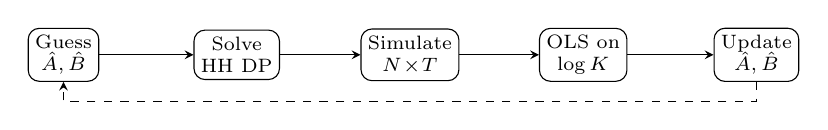
\begin{tikzpicture}[every node/.style={draw, rounded corners, font=\scriptsize, align=center, minimum height=0.55cm, inner sep=2.5pt}]
\node (n1) at (0,0)   {Guess\\$\hat A,\hat B$};
\node (n2) at (2.2,0) {Solve\\HH DP};
\node (n3) at (4.4,0) {Simulate\\$N\!\times\!T$};
\node (n4) at (6.6,0) {OLS on\\$\log K$};
\node (n5) at (8.8,0) {Update\\$\hat A,\hat B$};
\draw[->,>=stealth] (n1) -- (n2);
\draw[->,>=stealth] (n2) -- (n3);
\draw[->,>=stealth] (n3) -- (n4);
\draw[->,>=stealth] (n4) -- (n5);
\draw[->,>=stealth,dashed] (n5.south) -- ++(0,-0.25) -| (n1.south);
\end{tikzpicture}
\end{center}
\vspace{-0.4em}
{\scriptsize\textit{DeepHAM / DEQN replace the OLS step with a neural network trained on simulated states.}}
\end{frame}

\begin{frame}{Limitations of moment approximation}
\begin{itemize}
\item Although remarkably accurate \emph{on average}, the moment approximation has weaknesses:
\medskip
\begin{itemize}
\item \emph{Specific functional form} for the law of motion is hard to choose ex ante.
\item \emph{Higher-order properties} of the distribution (welfare, inequality measures) require more moments.
\item \emph{Optimal-policy analysis} (designing fiscal/monetary intervention) needs derivatives of the value function with respect to the full distribution, not just moments.
\end{itemize}
\medskip
\item \textbf{The natural alternative}: let a neural network \emph{learn} which features of $\Gamma$ matter.
\medskip
\item This is exactly the DeepHAM / DEQN approach.
\end{itemize}
\end{frame}

%=============================================================================
\section{DeepHAM}

\begin{frame}{DeepHAM (Han, Yang \& E, 2021 preprint, arXiv:2112.14377; \emph{Quantitative Economics} 17:297--341, 2026)}
\begin{itemize}
\item DeepHAM solves the (finite-$N$, large-$N$) Krusell--Smith problem as a \textbf{Markov Nash equilibrium} among $N$ agents.
\medskip
\item Two neural networks:
  \begin{itemize}
  \item Value function $V(s;\theta^V)$ for individual states.
  \item Policy $\mathcal{C}(s;\theta^C)$ for individual savings/consumption.
  \end{itemize}
\medskip
\item Training alternates:
  \begin{enumerate}
  \item \textbf{Value step}: simulate under current policy, compute Monte Carlo target, do supervised regression on $\theta^V$.
  \item \textbf{Policy step}: solve agent $i$'s problem with all other agents fixed at the previous policy --- \emph{fictitious play}.
  \end{enumerate}
\medskip
\item This decomposition makes the high-dimensional joint problem tractable.
\end{itemize}
\end{frame}

\begin{frame}{DeepHAM: algorithm outline}
\textbf{Initialisation ($k=0$).} Initial policy $\mathcal{C}^{(0)}$, networks $\theta^{V,(0)}, \theta^{C,(0)}$.
\medskip

\textbf{$k$-th iteration:}
\begin{enumerate}
\item Prepare the stationary distribution $\mu(\mathcal{C}^{(k-1)})$ under the previous policy.
\medskip
\item Update the value network by supervised learning:
\[
\theta^{V,(k)} \in \arg\min_{\theta^V}\;
\mathbb{E}_\mu\!\left[\big(V(s_i;\theta^V) - \hat V_i\big)^2\right],
\]
with target $\hat V_i = \sum_{\tau=0}^{T_v-1}\beta^\tau u(c_\tau^i)$.
\medskip
\item Update the policy network by fictitious play:
\[
\theta^{C,(k)} \in \arg\max_{\theta^C}\;
\mathbb{E}_\mu\!\left[\sum_{t=0}^{T-1}\beta^t u(c_{i,t}) + \beta^T V(s_{i,T};\theta^{V,(k)})\right].
\]
\end{enumerate}
\end{frame}

\begin{frame}{DeepHAM: value function learning}
\begin{itemize}
\item Simulate the economy for $T_v$ periods under the current policy $\mathcal{C}^{(k-1)}$.
\medskip
\item For each sampled initial state $s_i$, record the realised consumption path and compute the discounted utility target
\[
\hat V_i \;=\; \sum_{\tau=0}^{T_v-1} \beta^{\tau}\, u(c_{i,\tau}).
\]
\medskip
\item Train $V(\cdot;\theta^V)$ as a regression on $\{(s_i, \hat V_i)\}$.
\medskip
\item This is exactly fitted-value Monte Carlo: standard supervised deep learning, no special algorithms required.
\end{itemize}
\end{frame}

\begin{frame}{DeepHAM: policy iteration via fictitious play}
\begin{itemize}
\item In round $\ell+1$, all agents' policies $\mathcal{C}^{(k,\ell)}$ are known. Agent $i$ improves \emph{best-responding} to the previous policy of all others:
\[
\mathcal{C}^{(k,\ell+1)} \in \arg\max_{\mathcal{C}}\;
\mathbb{E}_\mu\!\left[\,\tilde U_{i,T} + \beta^T V^{(k)}(s_{i,T})\,\right].
\]
\medskip
\item Optimisation is over the parameters of the policy network and runs by gradient ascent on a Monte Carlo sample of paths.
\medskip
\item \textbf{Why fictitious play?}
  \begin{itemize}
  \item Decouples the high-dimensional fixed-point problem.
  \item Empirically robust: even in non-convex problems, alternating best response converges to a Nash equilibrium under regularity conditions.
  \end{itemize}
\end{itemize}
\end{frame}

\begin{frame}{DeepHAM: computational graph}
\begin{center}
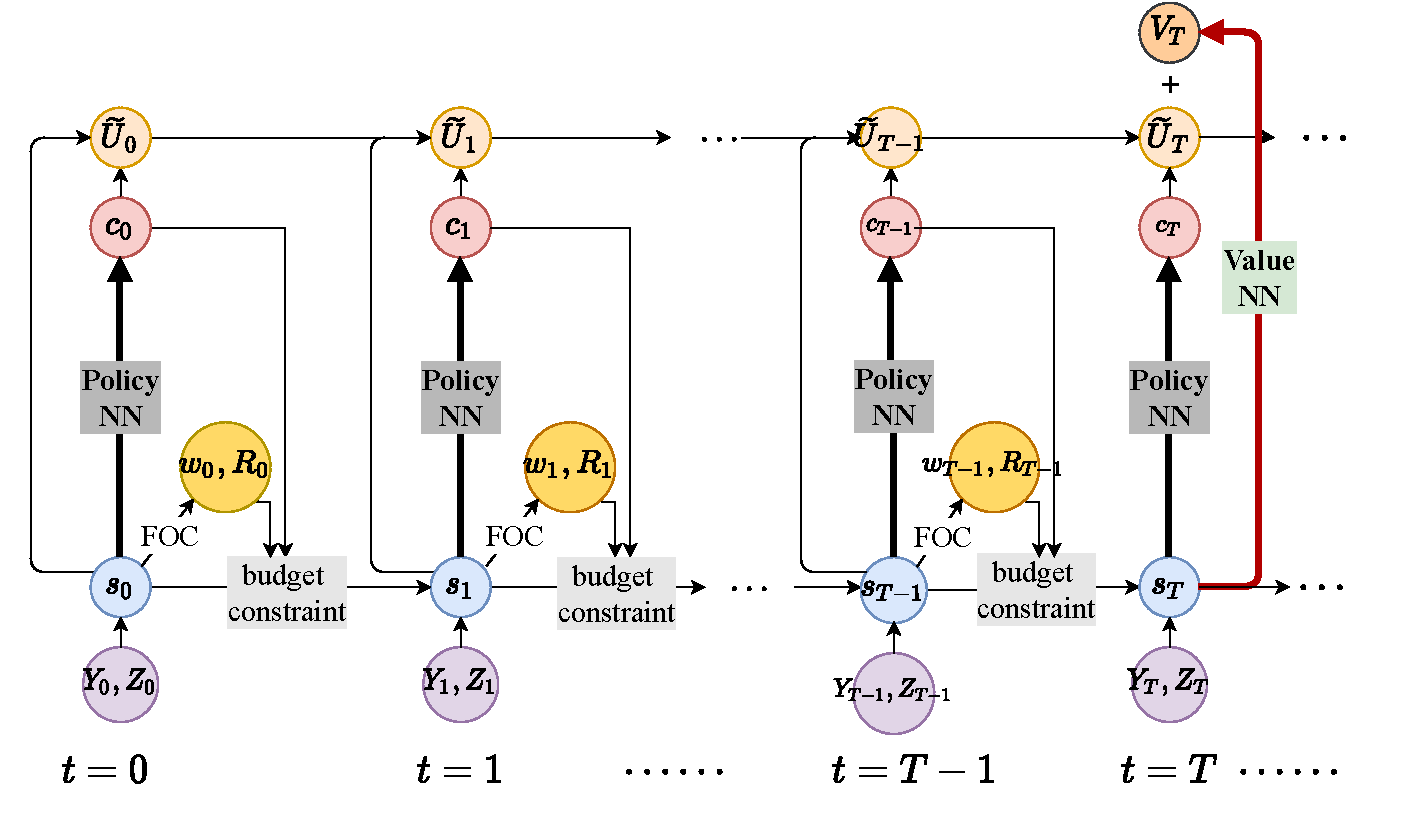
\includegraphics[width=0.85\textwidth]{KSwithDL_architecture_price_new}
\end{center}
\vspace{-0.4em}
\begin{itemize}
\item Inputs: individual state $s = (a_i, y_i, Z, \Gamma)$, with $\Gamma$ summarised by generalised moments.
\item Layers: feedforward MLP with multiple hidden layers.
\item Outputs: scalar consumption decision; budget constraint enforces $a' = R a + w y - c$.
\end{itemize}
\end{frame}

\begin{frame}{DL-based generalised moments}
\begin{itemize}
\item Instead of a fixed list of moments $\{m_1, m_2, \ldots\}$, DeepHAM lets the network \emph{learn} symmetry-preserving sufficient statistics:
\[
\bar Q_j(\Gamma) \;=\; \frac{1}{N} \sum_{i=1}^{N} Q_j(a_i),
\]
where $Q_1, \ldots, Q_J$ are basis functions parameterised by additional NN layers.
\medskip
\item Special case $Q_j(a) = a^j$ recovers the classical moments.
\medskip
\item Trained jointly with $V$ and $\mathcal C$, the learned moments adapt to the economic problem at hand.
\medskip
\item Symmetry across agents (the population is exchangeable) is enforced by averaging $Q_j$ across the cross section.
\end{itemize}
\end{frame}

\begin{frame}{Interpretation of generalised moments}
\begin{center}
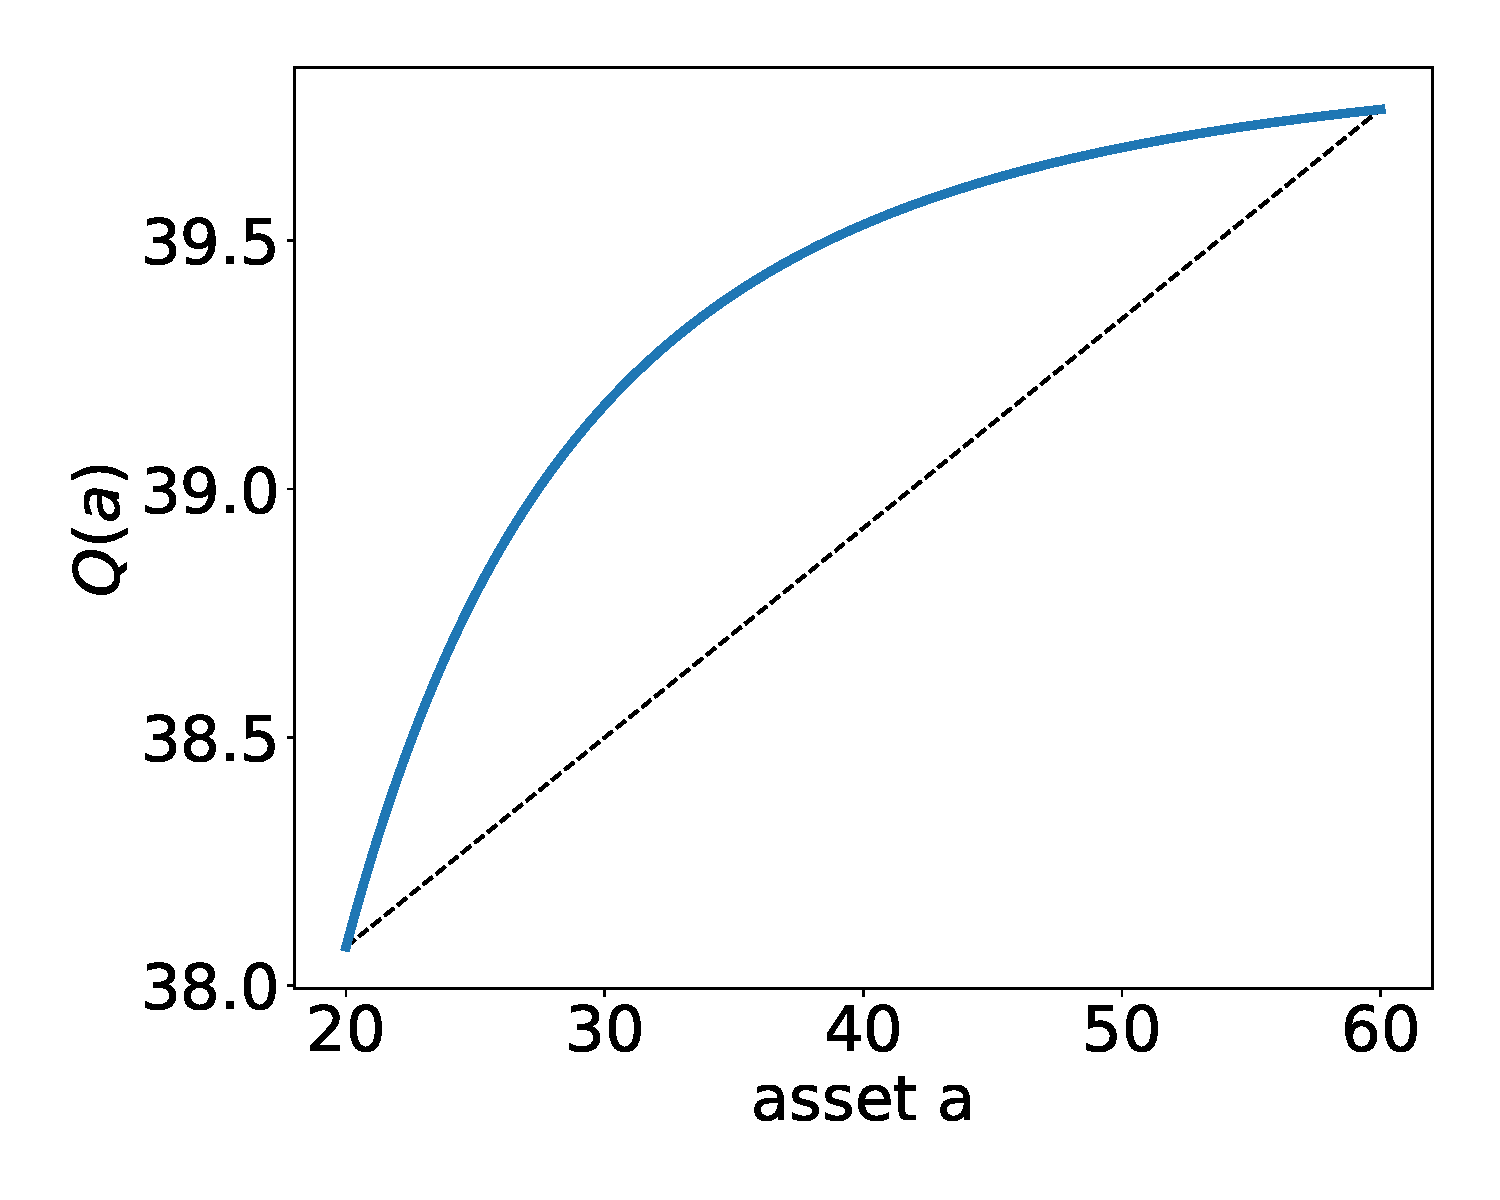
\includegraphics[width=0.85\textwidth]{KS_0fm1gm_v1_valuegmbasis_sub}
\end{center}
\vspace{-0.4em}
\begin{itemize}
\item Each panel: a learned basis function $Q_j(a)$ as a function of individual asset $a$.
\item The first basis function looks roughly linear ($\sim$ first moment); subsequent functions capture concavities and tail behaviour.
\item The network discovers, automatically, the features of $\Gamma$ that are relevant for forecasting.
\end{itemize}
\end{frame}

\begin{frame}{DeepHAM: training diagnostics}
\begin{center}
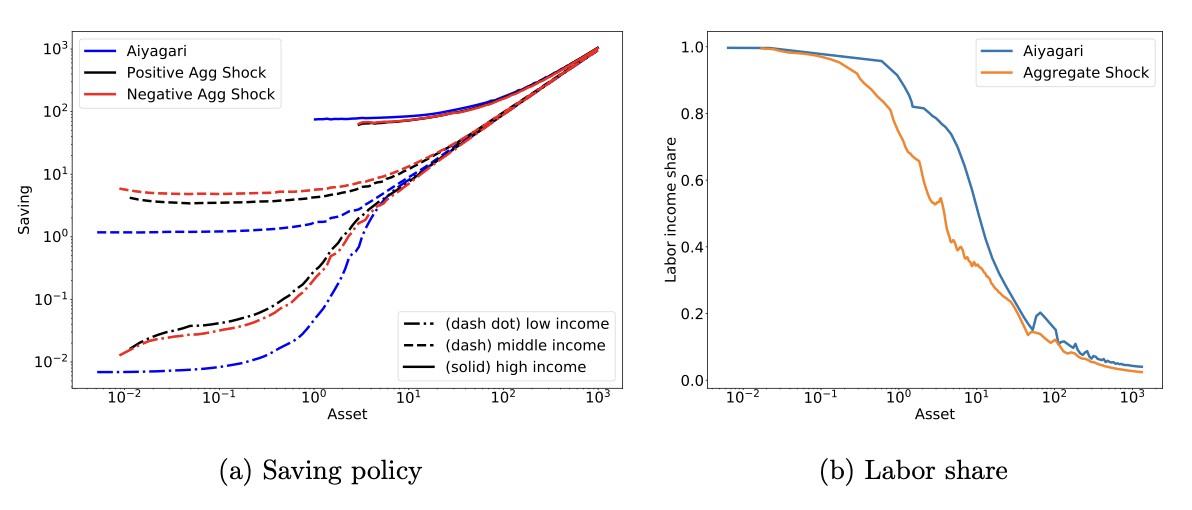
\includegraphics[height=3.6cm]{deepham}\hfill
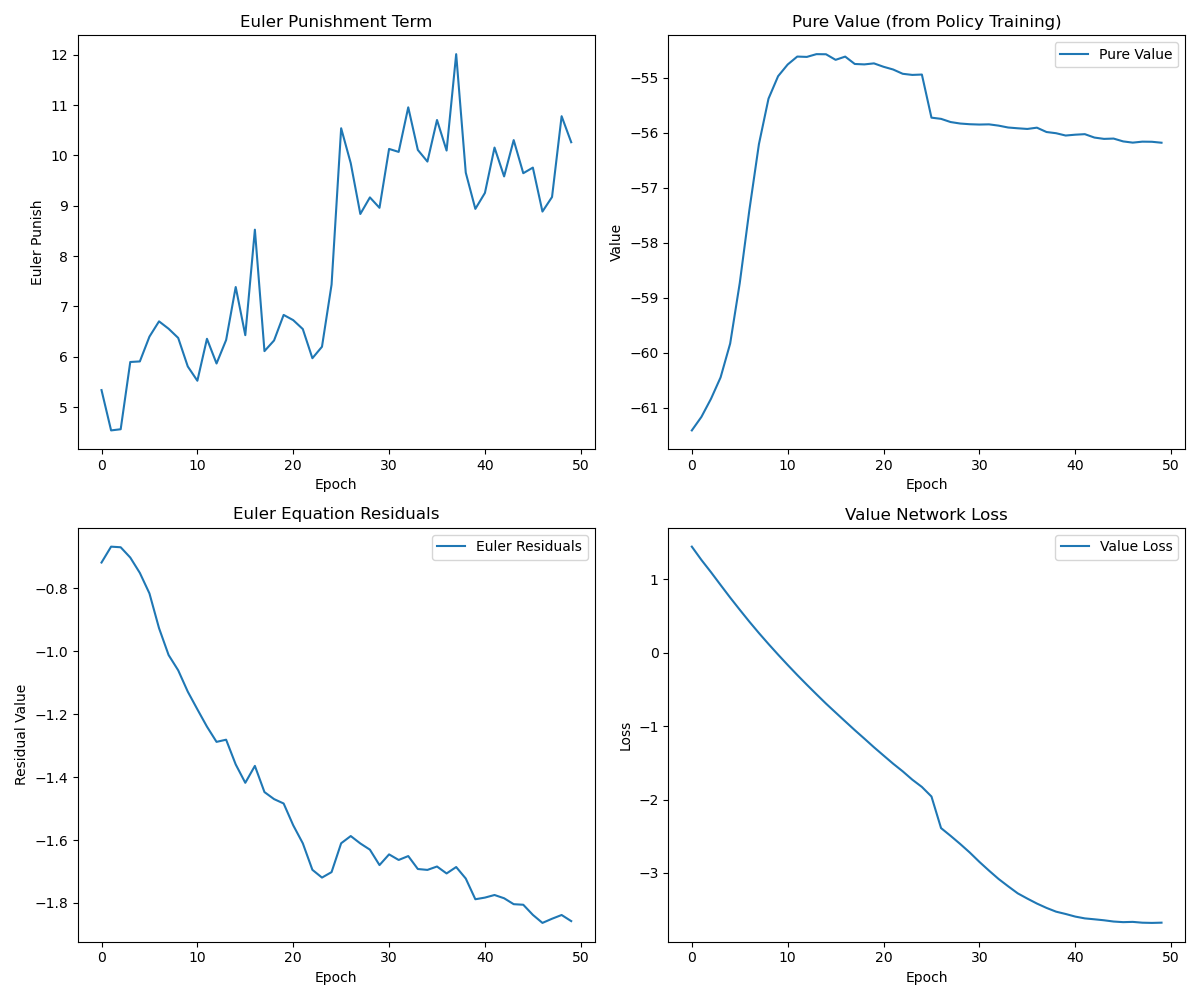
\includegraphics[height=3.6cm]{ddp_training_metrics}
\end{center}
\vspace{-0.3em}
\begin{itemize}
\item \emph{Left}: simulated cross section of capital under the trained policy.
\medskip
\item \emph{Right}: training loss curves over fictitious-play outer iterations; oscillation reflects the inner-regression vs.\ outer-policy-improvement decoupling.
\end{itemize}
\end{frame}

\begin{frame}{DeepHAM: learned policies}
\begin{center}
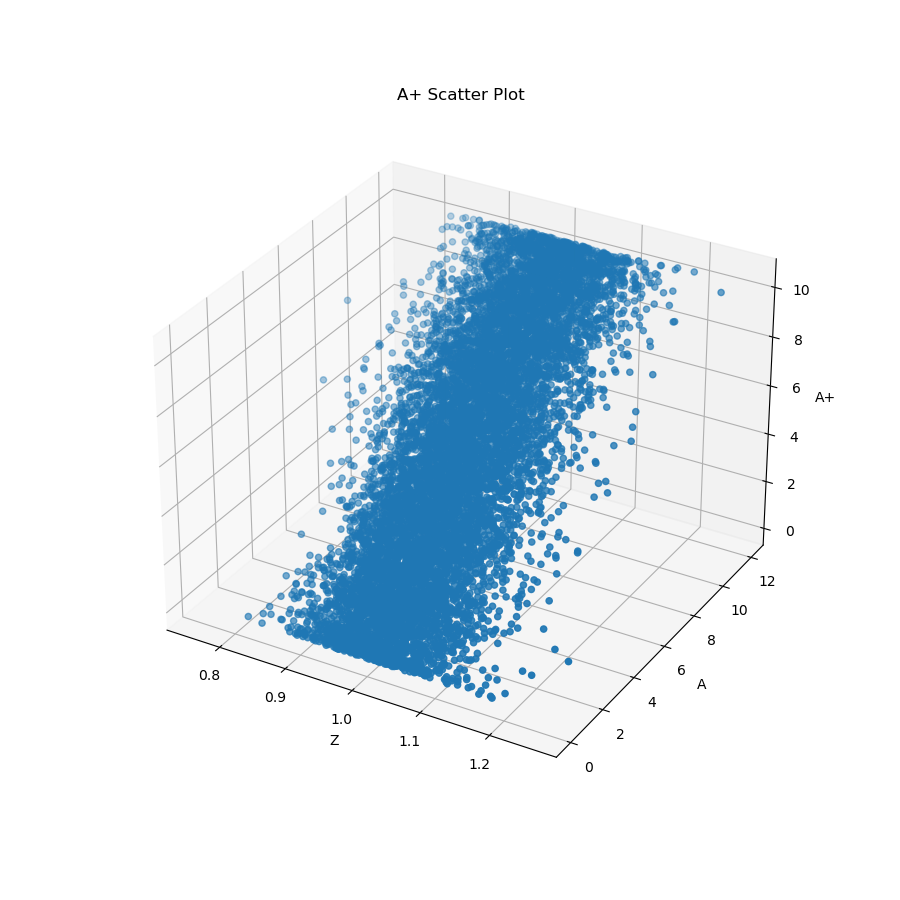
\includegraphics[height=4.2cm]{scatter_policy_a1}\hfill
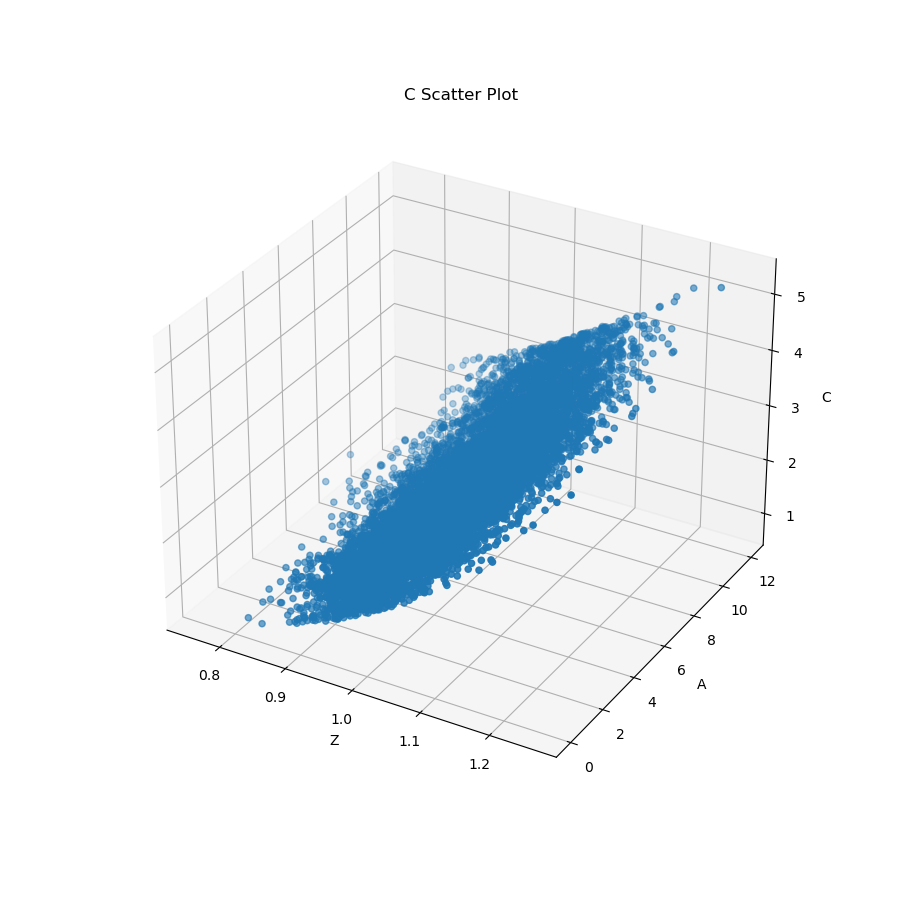
\includegraphics[height=4.2cm]{scatter_policy_c}
\end{center}
\vspace{-0.3em}
\begin{itemize}
\item \emph{Left}: learned savings policy, scattered across cross-section samples.
\item \emph{Right}: learned consumption policy, scattered across cross-section samples.
\item Gap to the classical KS-with-moments benchmark measures the value of DL-based generalised moments.
\end{itemize}
\medskip
\emph{Next (T4):} Deep Equilibrium Nets (a single Euler-loss network) and OLG with aggregate uncertainty.
\end{frame}

\end{document}
